\documentclass[answers]{exam}

%% Color
\usepackage[dvipsnames]{xcolor}

%% Language and font encodings
\usepackage{CJKutf8}
\usepackage[english,japanese]{babel}
\usepackage[utf8x]{inputenc}
\usepackage[T1]{fontenc}

%% Sets page size and margins
\usepackage[a4paper,margin=2cm]{geometry}

%% Useful packages
\usepackage{amsmath}
\usepackage{graphicx}
\usepackage{paralist}
\setlength\FrameSep{4pt}

\begin{document}
\begin{questions}

%%%%%%%%%%%%%%%%%%%%%%%%%
\question[10]{Copy your code comments here.}
\begin{framed}
\begin{compactenum}[A.]
	\item
    Create \texttt{nlayers\_enc} encoding layers using \texttt{add\_link}. There
    are two loops for adding layers because we create one encoder to pass over
    the sentence in order, and one to pass over the sentence in reverse order. 
  \item
    The encoding of a sentence is a matrix, each column of which is the
    concatenation of the hidden states of the forward and the backward encoder
    LSTMs at that position. Since both the LSTMs are sized \texttt{n\_units},
    the concatenation of these two hidden states is \texttt{2*n\_units}. 
  \item
    The method \texttt{set\_decoder\_state} will feed the encoder output into
    the decoder. The initial implementation takes the cell states and hidden
    state from the final LSTM of the encoder, and feeds them into the first LSTM
    of the decoder.  
  \item
    We are performing two encode operations because we are stepping through the
    sentence forwards and backwards at the same time -- see the call to
    \texttt{zip} above -- and we are encoding the `forwards' word using the
    forwards encoder, and the backwards word using the backwards encoder.  
  \item
    (\textcolor{red}{TODO add an example.})
    The loss is computed as the cross-entropy over two softmax distributions.
    The cross-entropy is a soft measure of how close the network got to the
    correct answer. Here it is used to find how close the predicted word
    (\texttt{predicted\_out}) was to the expected word
    (\texttt{next\_word\_var}).  
  \item
    The \texttt{add\_hook} function adds some code which is to be executed right
    after the computation of the gradient. The \texttt{GradientClipping}
    function will scale gradients down when their L2 norm goes over a certain
    threshold (here 5). 
\end{compactenum}
\end{framed}


%%%%%%%%%%%%%%%%%%%%%%%%%
\question[10]{Examine the parallel data and answer questions. (Plots may appear in the appendix.)}
\begin{framed}
\begin{compactenum}[1.]
	\item
    When looking at figures \ref{fig:toks} and \ref{fig:chars}, it seems as if
    English is a more productive language (more `meaning' with fewer symbols)
    when we measure sentence length in tokens, and Japanese is more productive
    when we measure it in characters. 
    Both metrics are unfair: Japanese uses logograms, which explains the
    high productivity using characters. However, it also uses a system of
    particles to mark e.g.\ subjects and objects, which are treated as separate
    words. Making matters worse, the tokeniser for Japanese seems to treat each
    hiragana as its own token, meaning long and common word endings such as
    `-\begin{CJK}{UTF8}{min}します\end{CJK}' are treated as three separate
    tokens. This partly explains the low of productivity using tokens.
    
    What our graphs \emph{do} show is that there is a linear correlation between
    sentence lengths in English and Japanese. This means that we can expect
    sentence length to change linearly when we translate, either as $|f| \approx
    1.42|e|$ (tokens) or as $|f| \approx 0.42|e|$ (characters). 
  \item
    In total, there are 97643 and 143581 tokens in the English and Japanese
    data, respectively.
  \item
    There are 7217 and 8246 word types/unique tokens in the English and Japanese
    data, respectively.
  \item
  \item
  \item
\end{compactenum}
\end{framed}


%%%%%%%%%%%%%%%%%%%%%%%%%
\question[10]{What language phenomena might influence what you observed above?}
\begin{framed}
\emph{Your answer here.}
\end{framed}


%%%%%%%%%%%%%%%%%%%%%%%%%
\question[10]{Answers to questions about sampling, beam search, and dynamic programming.}
\begin{framed}
\begin{compactenum}[1.]
	\item
    \item
    \item
\end{compactenum}
\end{framed}


%%%%%%%%%%%%%%%%%%%%%%%%%
\question[10]{Experiment with changes to the model, and explain results.}
\begin{framed}
\emph{Your answer here.}
\end{framed}


%%%%%%%%%%%%%%%%%%%%%%%%%
\question[10]{Implement dropout, and explain the results.}
\begin{framed}
\emph{Your answer here.}
\end{framed}


%%%%%%%%%%%%%%%%%%%%%%%%%
\question[20]{Implement attention. This question will be evaluated on the basis of your code.}

\question[10]{Explain the results of implementing attention.}
\begin{framed}
\emph{Your answer here}
\end{framed}

%%%%%%%%%%%%%%%%%%%%%%%%%
\question[10]{Explain what you observe with attention. (Figures may appear in an appendix.)}
\begin{framed}
\emph{Your answer here}
\end{framed}
\end{questions}

\noindent \hrulefill

\clearpage

\begin{figure}
  \centering
  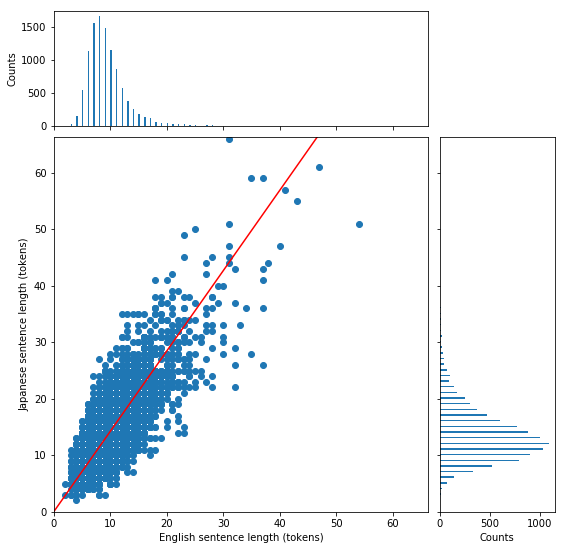
\includegraphics[width=\linewidth]{fig-toks}
  \caption[Sentence lenths (tokens)]%
  {Distribution of and correlation between Japanese and English sentence lengths (tokens)}
  \label{fig:toks}
\end{figure}

\begin{figure}
  \centering
  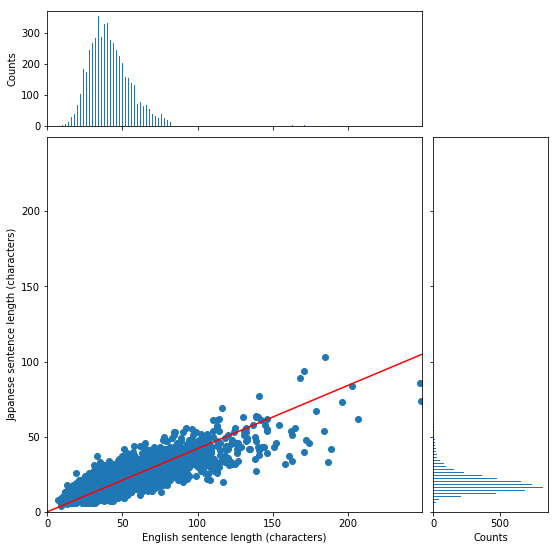
\includegraphics[width=\linewidth]{fig-chars}
  \caption[Sentence lenths (characters)]%
  {Distribution of and correlation between Japanese and English sentence lengths (tokens)}
  \label{fig:chars}
\end{figure}

\end{document}